\Tsec{Билет №3}

\begin{leftrules}
Генерация второй оптической гармоники. Понятие фазового синхронизма. Способ выполнения условия фазового синхронизма. Расчет угла фазового синхронизма при ГВГ.
\end{leftrules}


\textbf{Генерация второй гармоники}. Пусть в квадратично-нелинейный диэлектрик входит световая волна на частоте $\omega$. Тогда 
\begin{equation*}
    \vc{P}^{\text{кв}} = \frac{1}{4} \chi[\vc{e}, \vc{e}] (A e^{i (\omega t - \smallvc{k} \smallvc{r})} + \cc)^2 = \frac{1}{4} \chi[\vc{e}, \vc{e}] \left(
        A^2 e^{i (2 \omega t - 2 \smallvc{k} \smallvc{r})} + \bar{A}^2 e^{i(2 \smallvc{k} \smallvc{r} - 2 \omega t)} + 2 A \bar{A}
    \right).
\end{equation*}
% Засовывая в $\chi$ сумму двух волн на частоте $\omega_1$ и $\omega_2$ находим, что будут появляться волны на часоте $\omega_1 + \omega_2$ и $\omega_1 - \omega_2$.


\textbf{Intro}. Представим исходную волну и волну второй гармоники в виде
\begin{align*}
    E_\omega &= A_\omega \cos(\omega t - k z), \\
    E_{2 \omega} &= A_{2 \omega} \cos(2 \omega t - Kz).
\end{align*}
Считая $n[\omega] = \sqrt{\varepsilon[\omega]}$ и $n[2 \omega] = \sqrt{\varepsilon[2\omega]}$, находим
\begin{equation*}
    v_\omega = \frac{c}{n[\omega]} = \frac{\omega}{k_\omega},
    \hspace{5 mm} 
    v_{2\omega} = \frac{c}{n[2\omega]} = \frac{2\omega}{k_{2\omega}},
    \hspace{0.5cm} \Rightarrow \hspace{0.5cm}
     \boxed{k_{2\omega}-2k_{\omega} = \Delta k},
\end{equation*}
где $\Delta k$ -- \textit{волновая расстройка}. 


\textbf{Интерференция}. Исходная волна вызовет волну квадратичной поляризованности
\begin{equation*}
    P_{2 \omega} = \frac{1}{2} \chi[\vc{e}, \vc{e}] A_\omega^2 \cos(2 \omega t - 2 k z).
\end{equation*}
Рассмотрим две точки: $z$ и $z'$, пусть фаза волны в $z'$:
\begin{equation*}
    \Phi(z') = 2 \omega t - 2 k_\omega z'.
\end{equation*}
Тогда в точке $z$ фаза переизлученной световой волны будет
\begin{equation*}
    \varphi(z') = \Phi(z) - k_{2 \omega} (z-z') = 2 \omega t - k_{2 \omega} z + \Delta k z'.
\end{equation*}
Результирующая волна второй гармони есть результат интерференции волн, переизлученных в различных точках $z'$ на промежутку от $z' = 0$  дл $z' =z$:
\begin{equation*}
    E_{2 \omega} = A \int_{0}^{z}  \cos(\varphi[z']) \d z' = A \int_{0}^{z}  \cos(2 \omega t - K z + \Delta k z') \d z'.
\end{equation*}
Откуда находим, что
\begin{equation*}
    E_{2 \omega} = \frac{A}{\Delta k} \left(
        \sin(2 \omega t - k_{2 \omega} z + \Delta k z) - \sin(2 \omega t - k_{2 \omega} z)
    \right) = \frac{2 A}{\Delta k} \sin\left(\frac{\Delta k z}{2}\right) \cos\left(
        2 \omega t - k_{2 \omega} z + \frac{\Delta k z}{2}
    \right),
\end{equation*}
а значит амплитуда второй гармоники в точке $z$:
\begin{equation*}
    A_{2 \omega} (z) = \frac{2 A}{\Delta k} \sin \frac{\Delta k z}{2},
    \hspace{0.5cm} \Rightarrow \hspace{0.5cm}
    A_{2 \omega}^{\text{max}} \Leftrightarrow \boxed{k_{2 \omega} = 2 k_{\omega}},
\end{equation*}
так и приходим к условию \textit{фазового синхронизма}.

\textbf{Достижение фазового синхронизма}. Для отрицательного одноосного кристалла
\begin{equation*}
    \frac{n_z^2}{n_o^2} + \frac{n_x^2}{n_e^2} =1,
    \hspace{0.5cm} \Rightarrow \hspace{0.5cm}
    n_e [\theta] = \frac{n_o n_e}{\sqrt{n_o^2 - (n_o^2-n_e^2) \cos^2 \theta}},
\end{equation*}
так что можем добиться $n_o [\omega] = n_e[2 \omega]$, для некоторого $\theta$:
\begin{equation*}
    \frac{1}{n_e^2[2 \omega, \theta]} = \frac{\cos^2 (\theta)}{n_o^2 [2 \omega]} + \frac{\sin^2(\theta)}{n_e^2 [2\omega]} = \frac{1}{n_0^2[\omega]},
\end{equation*}
что прекрасно видно на графике.
\begin{figure}[h]
    \centering
    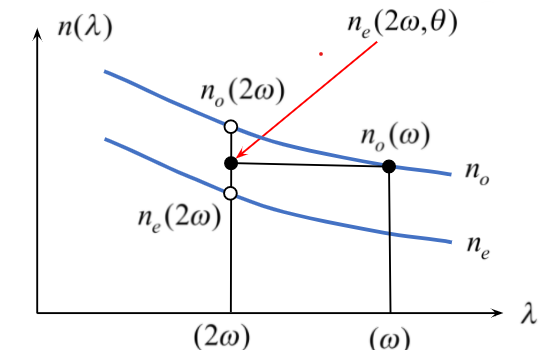
\includegraphics[width=0.3\textwidth]{figures/3_1.png}
    \caption{Достижение фазового синхронизма}
    %\label{fig:}
\end{figure}
